\begin{newpart}{MK: re-read; @FR: correct the last sentences.}
  The immediate application of the Jupyter/MMT integration presented in this paper is interacting with MMT in a REPL.
  The MMT tool ecosystem only really supported IDE-interaction with MMT libraries via JEdit and (recently) IntelliJ IDEa plugins. 
  While the MMT system provides a simple shell for interaction, this was only used for configuration and setup of the MMT process.
  We anticipate that the REPL-like interaction will feel more natural for users of interactive theorem provers and computer algebra systems.
  Even for the new MathScheme-style of specifying theory graph libraries via theory combinators~\cite{RabSha:????19}, e.g. 
\begin{lstlisting}[mathescape]
semigroup = extend magma by {assoc: $\vdash\forall{a,b,c}:G. a\circ (b\circ c) = (a\circ b)\circ c $}
\end{lstlisting}
  is well-suited to development/experimentation in a REPL followed by generating an OMDoc file from the recorded notebook.
\end{newpart}

\subsection{Towards a Virtual Research Environment based on the Math-in-the-Middle Paradigm}


Another direct application is in the context of the OpenDreamKit project, which integrates various independently developed computational engines into a mathematical virtual research environment following the Math-in-the-Middle (MitM) approach~\cite{DehKohKon:iop16}.
This uses the MMT language for formalizing mathematical background knowledge (which we store in MathHub documents of type MMT) and the MMT system for integrating computation tools.
Therefore, Jupyter-MMT notebooks can serve as a unified user interface for MitM systems.

For example, consider the theory\footnote{Available at \url{https://gl.mathhub.info/ODK/lmfdb/blob/master/source/schemas/tutorial_example.mmt}}  in Figure~\ref{fig:hecke}, which serves as our standard example for the interaction between MMT and LMFDB (a large database of mathematical objects that was integrated with MMT in previous deliverables of OpenDreamKit).
We can now rewrite it as a notebook.

\begin{wrapfigure}{r}{0.7\textwidth}
  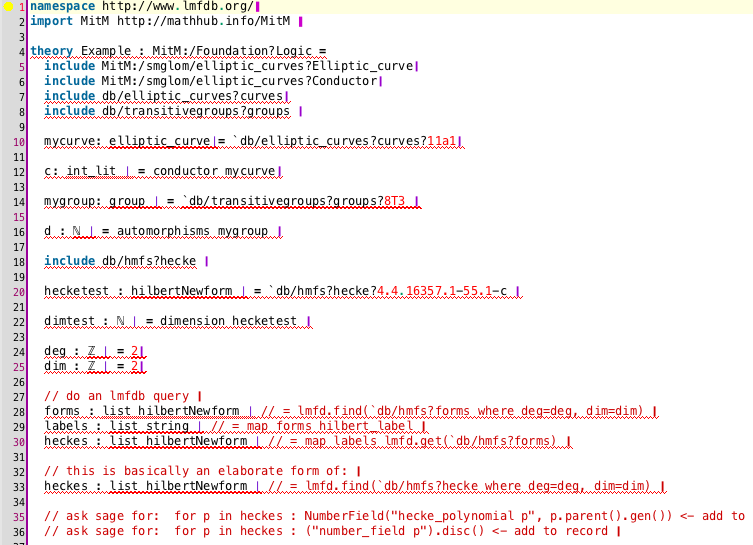
\includegraphics[width=0.7\textwidth]{../D4.11/hecke}
  \caption{A Theory for LMFDB/MMT Interaction}\label{fig:hecke}
\end{wrapfigure}
A screenshot of the resulting notebook, as displayed by a Jupyter server running our MMT kernel, is shown in Figure~\ref{fig:lmfdbexample}.
The selected declaration of \texttt{mycurve} accesses the elliptic curve \texttt{11a1} that is stored in LMFDB.
When the Jupyter kernel for MMT processes this command, the bottom layer of the kernel dynamically retrieves this curve from LMFDB and builds from it an object of type \texttt{elliptic\_curve} in the MitM ontology.

\begin{figure}[ht]\centering
  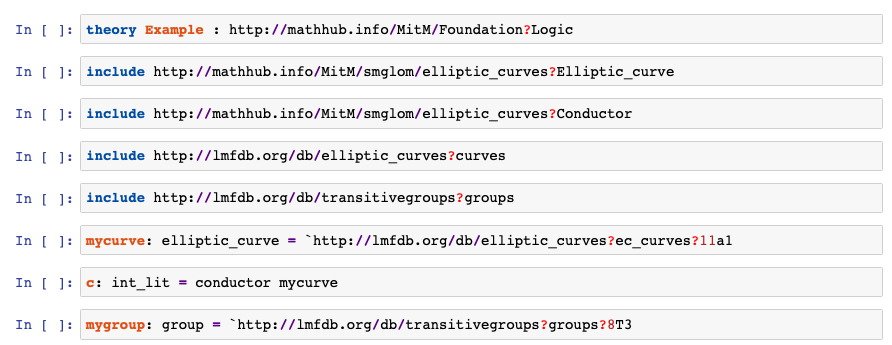
\includegraphics[width=0.9\textwidth]{screenshots/heckenb}
  \caption{The Beginning of the Notebook for the theory from Figure~\ref{fig:hecke}}\label{fig:lmfdbexample}
\end{figure}

\subsection{Domain specific applications: MoSIS}

\begin{figure}[ht]\centering
  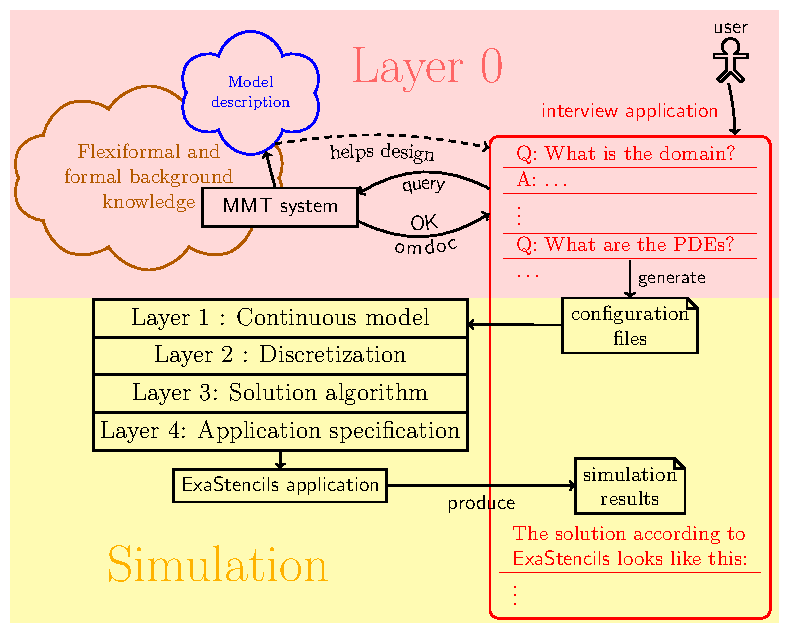
\includegraphics[width=0.6\textwidth]{../D4.11/proto}
  \caption{MoSIS Information Architecture}\label{fig:prototype}
\end{figure}

Our second case study addresses a \emph{knowledge gap} that is commonly encountered in computational science and engineering:
To set up a simulation, we need to combine domain knowledge (usually in terms of physical principles), model knowledge (e.g., about suitable partial differential equations) with simulation (i.e., numerics/computing) knowledge.
In pre-VRE practice, this is resolved by intense collaboration between experts, which incurs non-trivial translation and communication overheads.
In OpenDreamKit, we propose an alternate solution based on mathematical knowledge management techniques.
A detailed description was published as \cite{PolKohKoe:kacse18}.

Concretely, we use a Jupyter notebook that has access to an MMT theory graph on MathHub.info.  Our Jupyter/MMT/Mathhub integration enabled building an interview application that hides these mathematical details from the user.

% \begin{figure}[ht]
%   \fbox{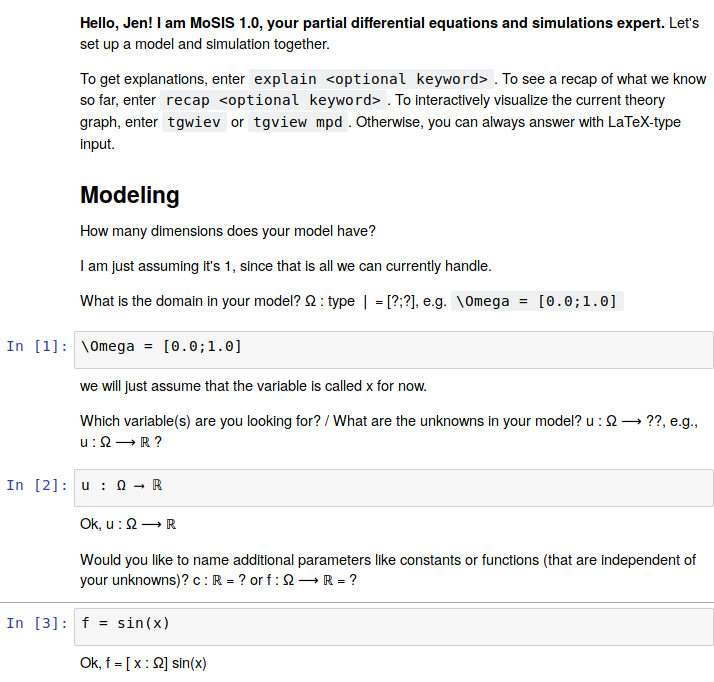
\includegraphics[width=0.8\textwidth]{../D4.11/Screenshot_interview}}
%   \caption{Beginning of a Dialogue in MoSIS}\label{fig:int_begin}
% \end{figure}

% \begin{figure}[h!p]\centering
%   \begin{turn}{-90}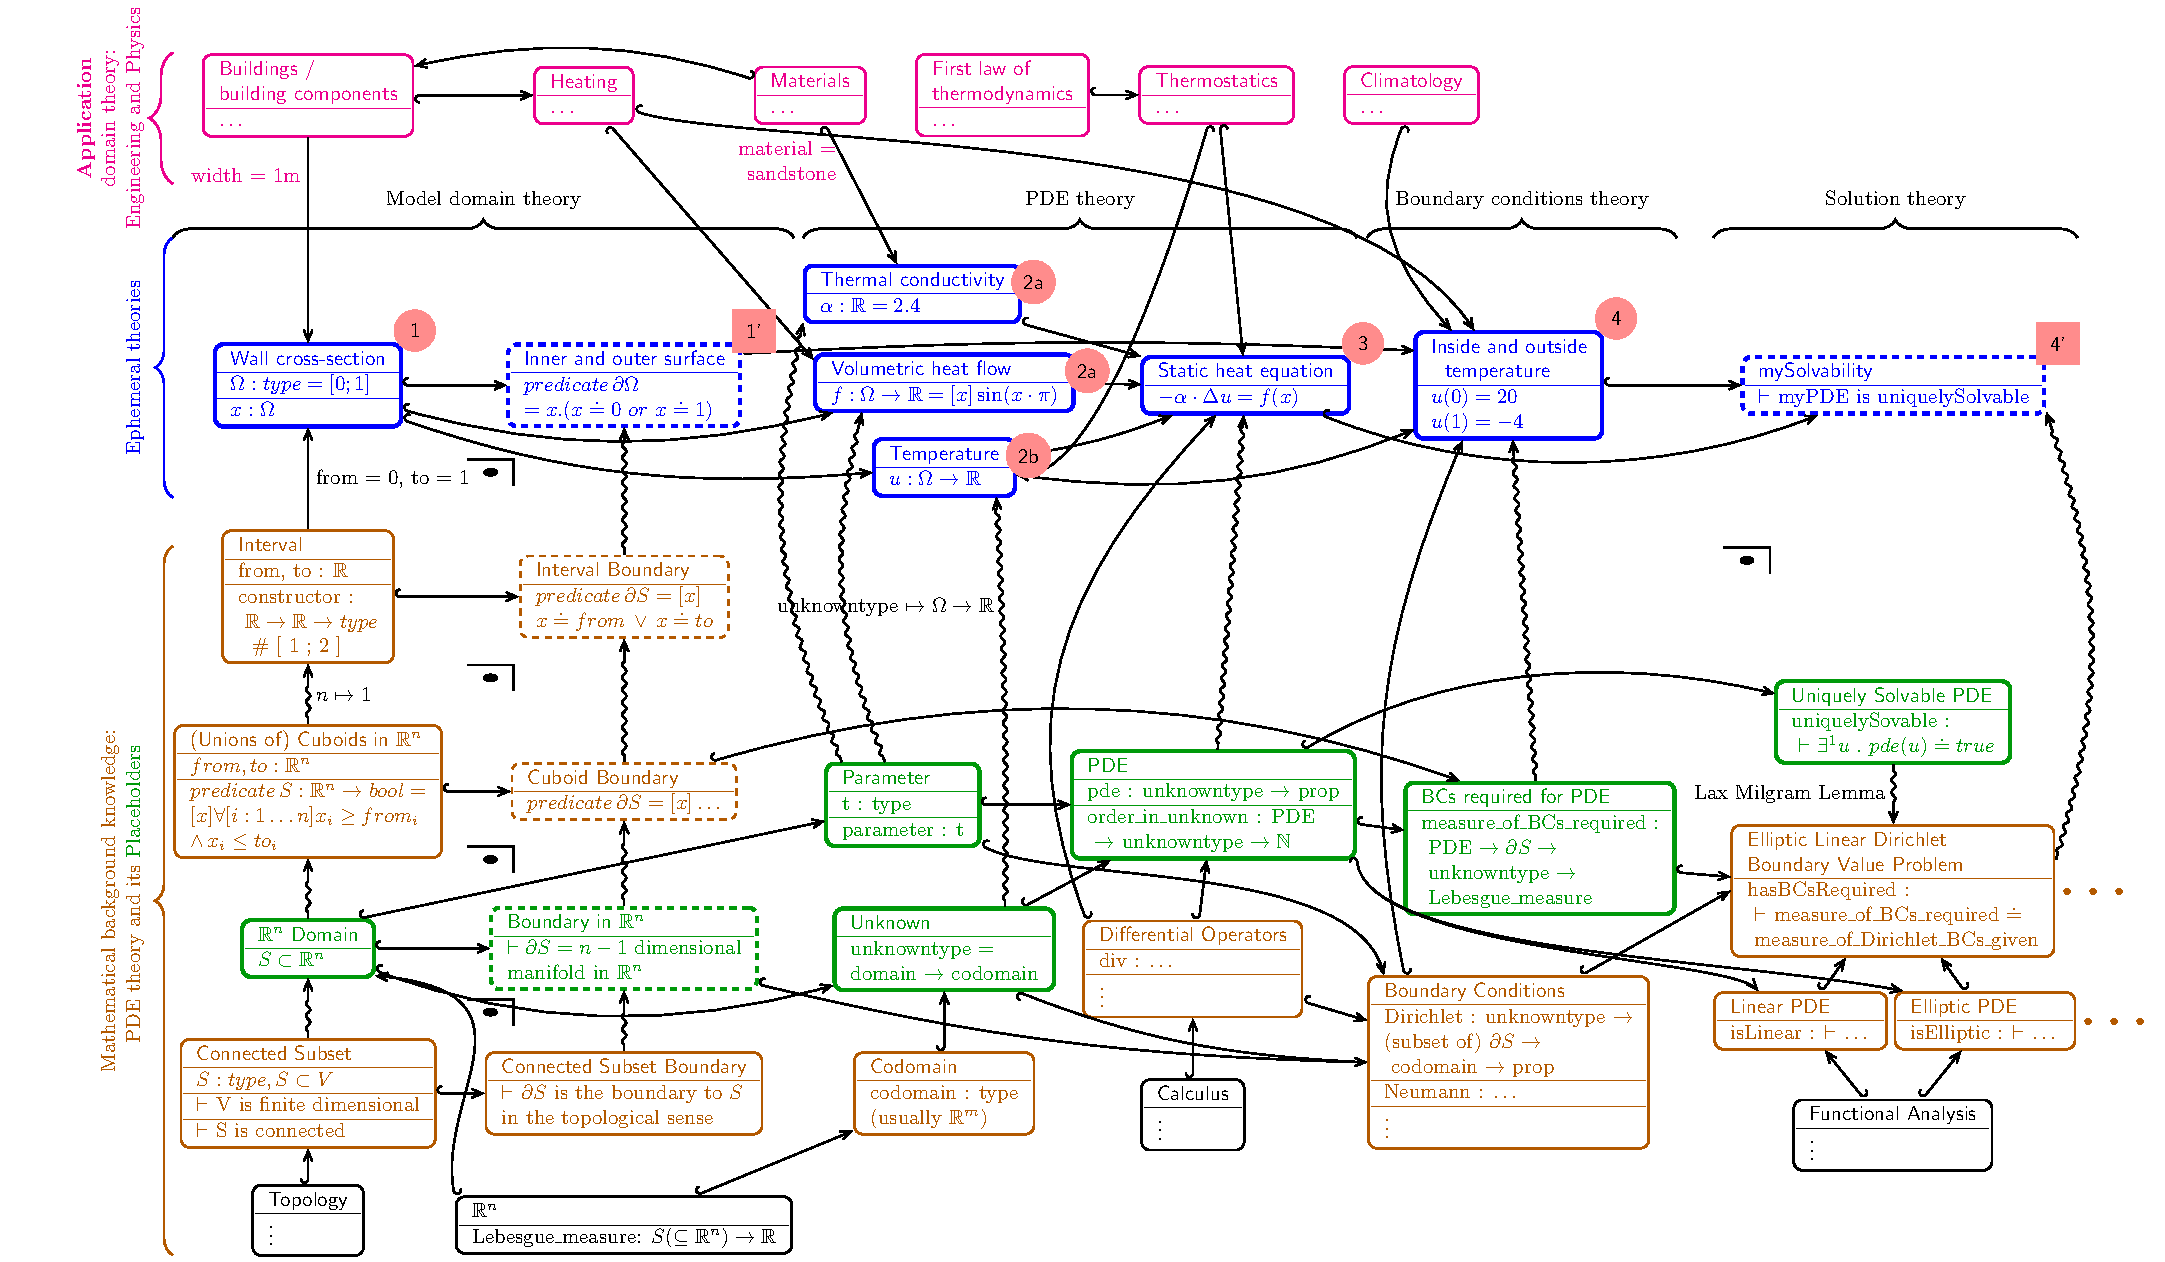
\includegraphics[width=0.95\textheight]{pde-theory}\end{turn}
%   \caption{Theory Graph for the MoSIS Case Study}\label{fig:pde-theory}
% \end{figure}

Based on this theory graph, we built a targeted knowledge acquisition dialog that supports the formalization of domain knowledge, combines it with simulation knowledge and finally drives a simulation run --- all integrated into a Jupyter Notebook.
Figure~\ref{fig:prototype} shows the general architecture:
The left side shows the simulation engine \textsf{ExaStencils}~\cite{exastencils.on} and the MMT system that acts as the theory graph interface.
The right hand side shows the interview --- a Jupyter notebook --- as the active document and how it interacts with the MMT kernel.
The user only sees the notebook.
She answers the knowledge acquisition questions presented by MoSIS until MoSIS can generate a configuration file for ExaStencils.
The latter builds efficient code from it through the ExaSlang layers and computes the results and visualizations, which MoSIS in turn incorporates into the notebook. 

%%% Local Variables:
%%% mode: latex
%%% mode: visual-line
%%% fill-column: 5000
%%% TeX-master: "paper"
%%% End:

%  LocalWords:  MitM-Based Formalized formalizing Jupyter-MMT ednote summarize centering includegraphics textwidth Jupyter fig:lmfdbexample texttt mycurve texttt textbf lmfdb_example emph PolKohKoe:kacse18 fig:pde-theory fbox textheight pde-theory formalization textsf exastencils.on visualizations newpart JEdit DehKohKon:iop16
